\chapter{Problema 1}

\section{1759 - Cubo}

\subsection{Enunciado}

En un futuro no muy lejano las personas buscar�n juegos cada vez m�s peligrosos
para jugar. Despu�s de ultra-ligeros y el bungee-jumping las personas necesitan
juegos donde sus actividades mentales tambi�n se pongan a prueba. Este es el
caso del juego llamado 'cubo', inventado en Nueva Zelanda. En algunos lugares
tambi�n es conocido por su nombre japon�s: sokoban.

Considere un laberinto de dos dimensiones compuesto de casillas cuadradas, donde
cada una est� libre o est� ocupada por una piedra. En cada paso, puede salir de
una casilla y moverse a otra casilla vecina (es decir, arriba, abajo, izquierda y
derecha) libre. Usted est� ocupando una de las casillas libres de este laberinto.

\begin{figure}[H]
\centering
\label{ej1_sokoban}
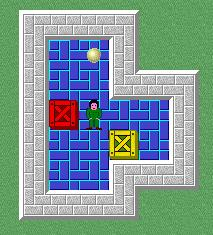
\includegraphics[scale=0.8]{./graficos/ej1/sokoban.jpg}
\caption{Ejemplo del juego}
\end{figure}

Una casilla del laberinto contiene una pila de cajas. La pila puede ser movida 
de una casilla i a una casilla k (por ejemplo, k = i+1), vecina de i, en la
direcci�n ik si usted estuviera en la casilla j (aqu� j = i-1), vecina de i, y
la direcci�n ik es igual a la direcci�n ji. Una caja no puede ser movida de
ninguna otra manera (es decir, no se puede tirar de la caja). As� que si la
caja termina en una esquina del laberinto no podr� moverla nuevamente.
Por �ltimo, tenga en cuenta que en cada empuj�n de la caja usted da un paso, y
que lo inverso no es necesariamente cierto.

Una de las casillas vac�as est� marcada como la casilla final. Su tarea es
llevar la caja a la casilla final a trav�s de una serie de pasos y empujones de
la caja. Como la caja es pesada, quiere realizar el menor n�mero posible de
empujones de la caja.

Tenga en cuenta que en el juego de la vida real existe la posibilidad de que
pueda ser aplastado por la caja, haciendo que todo mucho m�s divertido.

\textbf{Input:}

El archivo de entrada se compone de varias instancias. Cada instancia se inicia
con una l�nea que contiene dos entero r y c (ambos menores o iguales que 20) que
representando el n�mero de filas y columnas del laberinto.

Luego se les proporcionan r l�neas, cada una con c caracteres. Cada caracter
describe una casilla del laberinto. Una casilla ocupada por una piedra se indica
por \# y una casilla vac�a est� representada por un '.' (sin las comillas). Su
posici�n de partida se indica con S, la posici�n inicial de la caja est� indicada
por B y la posici�n final de la caja se indica por el T.

La entrada termina cuando r = c = 0.

\textbf{Output:}

Para cada laberinto, imprima en primer lugar el n�mero de instancia, como se
muestra en la salida de ejemplo siguiente. Si no es posible llevar el cuadro
a su posici�n final, escriba una l�nea conteniendo 'Impossivel'.
De lo contrario, deber� imprimir dos enteros x e y, donde x indica el n�mero
de movimientos (pasos + empujones) e y el numero de empujones de una secuencia
que hace que lleve la cada hasta la posici�n final. El n�mero de empujones debe
ser m�nimo. Si hay m�s de una posible secuencia que utiliza un n�mero m�nimo de
empujes, el n�mero total de movimientos debe ser m�nimo.
Imprima una l�nea en blanco despu�s de cada instancia.

\textbf{Url:}

\href{https://br.spoj.pl/problems/CUBO/}{Problema de cubo}

\subsection{Modelo}

\subsection{Soluci�n}

\subsection{Detalles de implementaci�n}

\subsection{C�lculo de complejidad}